\begin{frame}{Το σύστημα \texttt{fsm2}}



  \noindent\makebox[\linewidth][c]{%
  \begin{minipage}{\linewidth}
    \begin{minipage}{0.45\linewidth}
      \begin{figure}
        

\tikzset{every picture/.style={line width=0.75pt}} %set default line width to 0.75pt

\begin{tikzpicture}[x=0.75pt,y=0.75pt,yscale=-0.5,xscale=0.5]
%uncomment if require: \path (0,402); %set diagram left start at 0, and has height of 402

\draw    (138.5,36.83) -- (138.5,69.67) -- (138.5,100.23) ;
\draw    (301.19,39.17) -- (301.19,83.17) ;
\draw [shift={(301.19,85.17)}, rotate = 270] [color={rgb, 255:red, 0; green, 0; blue, 0 }  ][line width=0.75]    (10.93,-3.29) .. controls (6.95,-1.4) and (3.31,-0.3) .. (0,0) .. controls (3.31,0.3) and (6.95,1.4) .. (10.93,3.29)   ;
\draw    (301.19,112.69) -- (301.19,141.69) ;
\draw [shift={(301.19,143.69)}, rotate = 270] [color={rgb, 255:red, 0; green, 0; blue, 0 }  ][line width=0.75]    (10.93,-3.29) .. controls (6.95,-1.4) and (3.31,-0.3) .. (0,0) .. controls (3.31,0.3) and (6.95,1.4) .. (10.93,3.29)   ;
\draw    (157.93,36.83) -- (157.93,157.93) -- (157.93,335.33) ;
\draw    (176.5,36.83) -- (176.5,336.23) ;
\draw    (161.5,100.23) -- (138.25,100.23) ;
\draw    (176.5,157.93) -- (157.93,157.93) ;
\draw    (301.19,169.69) -- (301.19,198.69) ;
\draw [shift={(301.19,200.69)}, rotate = 270] [color={rgb, 255:red, 0; green, 0; blue, 0 }  ][line width=0.75]    (10.93,-3.29) .. controls (6.95,-1.4) and (3.31,-0.3) .. (0,0) .. controls (3.31,0.3) and (6.95,1.4) .. (10.93,3.29)   ;
\draw    (176.5,157.93) -- (200.67,157.93) ;
\draw [shift={(202.67,157.93)}, rotate = 180] [color={rgb, 255:red, 0; green, 0; blue, 0 }  ][line width=0.75]    (10.93,-3.29) .. controls (6.95,-1.4) and (3.31,-0.3) .. (0,0) .. controls (3.31,0.3) and (6.95,1.4) .. (10.93,3.29)   ;
\draw    (301.19,227.69) -- (301.19,256.69) ;
\draw [shift={(301.19,258.69)}, rotate = 270] [color={rgb, 255:red, 0; green, 0; blue, 0 }  ][line width=0.75]    (10.93,-3.29) .. controls (6.95,-1.4) and (3.31,-0.3) .. (0,0) .. controls (3.31,0.3) and (6.95,1.4) .. (10.93,3.29)   ;
\draw    (301.19,288.69) -- (301.19,317.69) ;
\draw [shift={(301.19,319.69)}, rotate = 270] [color={rgb, 255:red, 0; green, 0; blue, 0 }  ][line width=0.75]    (10.93,-3.29) .. controls (6.95,-1.4) and (3.31,-0.3) .. (0,0) .. controls (3.31,0.3) and (6.95,1.4) .. (10.93,3.29)   ;
\draw    (301.19,345.69) -- (301.19,374.69) ;
\draw [shift={(301.19,376.69)}, rotate = 270] [color={rgb, 255:red, 0; green, 0; blue, 0 }  ][line width=0.75]    (10.93,-3.29) .. controls (6.95,-1.4) and (3.31,-0.3) .. (0,0) .. controls (3.31,0.3) and (6.95,1.4) .. (10.93,3.29)   ;
\draw    (157.93,276.99) -- (233.25,276.99) ;
\draw [shift={(235.25,277)}, rotate = 180] [color={rgb, 255:red, 0; green, 0; blue, 0 }  ][line width=0.75]    (10.93,-3.29) .. controls (6.95,-1.4) and (3.31,-0.3) .. (0,0) .. controls (3.31,0.3) and (6.95,1.4) .. (10.93,3.29)   ;
\draw    (157.93,335.99) -- (229.25,335.99) ;
\draw [shift={(231.25,336)}, rotate = 180] [color={rgb, 255:red, 0; green, 0; blue, 0 }  ][line width=0.75]    (10.93,-3.29) .. controls (6.95,-1.4) and (3.31,-0.3) .. (0,0) .. controls (3.31,0.3) and (6.95,1.4) .. (10.93,3.29)   ;
\draw    (176.5,214.88) -- (250.67,214.88) ;
\draw [shift={(252.67,214.9)}, rotate = 180] [color={rgb, 255:red, 0; green, 0; blue, 0 }  ][line width=0.75]    (10.93,-3.29) .. controls (6.95,-1.4) and (3.31,-0.3) .. (0,0) .. controls (3.31,0.3) and (6.95,1.4) .. (10.93,3.29)   ;
\draw    (429,157.93) -- (401.67,157.93) ;
\draw [shift={(399.67,157.93)}] [color={rgb, 255:red, 0; green, 0; blue, 0 }  ][line width=0.75]    (10.93,-3.29) .. controls (6.95,-1.4) and (3.31,-0.3) .. (0,0) .. controls (3.31,0.3) and (6.95,1.4) .. (10.93,3.29)   ;
%Shape: Rectangle [id:dp1523009551723873]
\draw  [dash pattern={on 0.84pt off 2.51pt}] (100.23,61.67) -- (502,61.67) -- (502,365) -- (100.23,365) -- cycle ;
\draw    (161.5,100.23) -- (190.67,100.23) ;
\draw [shift={(192.67,100.23)}, rotate = 180] [color={rgb, 255:red, 0; green, 0; blue, 0 }  ][line width=0.75]    (10.93,-3.29) .. controls (6.95,-1.4) and (3.31,-0.3) .. (0,0) .. controls (3.31,0.3) and (6.95,1.4) .. (10.93,3.29)   ;

% Text Node
\draw    (195.69,87.83) -- (406.69,87.83) -- (406.69,112.83) -- (195.69,112.83) -- cycle  ;
\draw (303.19,101.23) node   [align=left] {\tiny Εκτίμηση Προσανατολισμού};
% Text Node
\draw (214,146.83) node [anchor=north west][inner sep=0.75pt]   [align=left] {$ $};
% Text Node
\draw (133,17.83) node [anchor=north west][inner sep=0.75pt]   [align=left] {\tiny $\displaystyle \nu $};
% Text Node
\draw (147,17.83) node [anchor=north west][inner sep=0.75pt]   [align=left] {\tiny $\displaystyle \mathcal{S}_{R}$};
% Text Node
\draw (295.69,18.4) node [anchor=north west][inner sep=0.75pt]   [align=left] {\tiny $\displaystyle \hat{\bm{p}}$};
% Text Node
\draw (170,18.4) node [anchor=north west][inner sep=0.75pt]   [align=left] {\tiny $\bm{M}$};
% Text Node
\draw    (256.21,201.83) -- (346.21,201.83) -- (346.21,226.83) -- (256.21,226.83) -- cycle  ;
\draw (303.21,217.33) node   [align=left] {\tiny \texttt{scan\_map} };
% Text Node
\draw    (206.24,144.83) -- (396.24,144.83) -- (396.24,169.83) -- (206.24,169.83) -- cycle  ;
\draw (301.24,157.93) node   [align=left] {\tiny \ Πρόβα Εκτίμησης Θέσης \ };
% Text Node
\draw (325.69,116.33) node [anchor=north west][inner sep=0.75pt]   [align=left] {\tiny $\hat{\bm{P}}_{OE} = \text{OE}(\hat{\bm{p}})$};
% Text Node
\draw (326.69,173.33) node [anchor=north west][inner sep=0.75pt]   [align=left] {\tiny $\hat{\bm{P}}_{RPE} = \text{RPE}(\hat{\bm{P}}_{OE})$};
% Text Node
\draw    (237.69,262.83) -- (398.69,262.83) -- (398.69,288.83) -- (237.69,288.83) -- cycle  ;
\draw (235.69,266.83) node [anchor=north west][inner sep=0.75pt]   [align=left] {\tiny $\bm{C} = \text{CAER}(\mathcal{S}_R,\bm{\mathcal{S}}_V)$};
% Text Node
\draw (326.69,235.33) node [anchor=north west][inner sep=0.75pt]   [align=left] {\tiny $\bm{\mathcal{S}}_V$};
% Text Node
\draw    (234.54,320.83) -- (367.54,320.83) -- (367.54,345.83) -- (234.54,345.83) -- cycle  ;
\draw (303.04,335.33) node   [align=left] {\tiny Εκτίμηση Θέσης};
% Text Node
\draw (325.69,295.33) node [anchor=north west][inner sep=0.75pt]   [align=left] {\tiny $\hat{\bm{p}}_{C} \in \hat{\bm{P}}_{OE} : \text{CAER}(\mathcal{S}_R, \texttt{scan\_map}(\bm{M}, \text{RPE}(\hat{\bm{p}}_C))) = \min\{\bm{C}\}$};
% Text Node
\draw (295.69,383.33) node [anchor=north west][inner sep=0.75pt]   [align=left] {\tiny $\hat{\bm{p}}^{\prime}$};
% Text Node
\draw (433.33,148) node [anchor=north west][inner sep=0.75pt]   [align=left] {\tiny $I_T = 1$};


\draw (413.33,325.33) node [anchor=north west][inner sep=0.75pt]   [align=left] {\tiny $I_T = f(\nu)$};
\draw    (372,335.33) -- (403.67,335.3) ;
\draw [shift={(371.67,335.33)}] [color={rgb, 255:red, 0; green, 0; blue, 0 }  ][line width=0.75]    (10.93,-3.29) .. controls (6.95,-1.4) and (3.31,-0.3) .. (0,0) .. controls (3.31,0.3) and (6.95,1.4) .. (10.93,3.29)   ;

% Text Node
\draw (342.67,40) node [anchor=north west][inner sep=0.75pt]   [align=left] {\tiny Σύστημα Άπαξ Εκτίμησης Στάσης };


\end{tikzpicture}

      \end{figure}
    \end{minipage}
    \hfill
    \begin{minipage}{0.45\linewidth}
      \begin{figure}
        

\tikzset{every picture/.style={line width=0.75pt}} %set default line width to 0.75pt

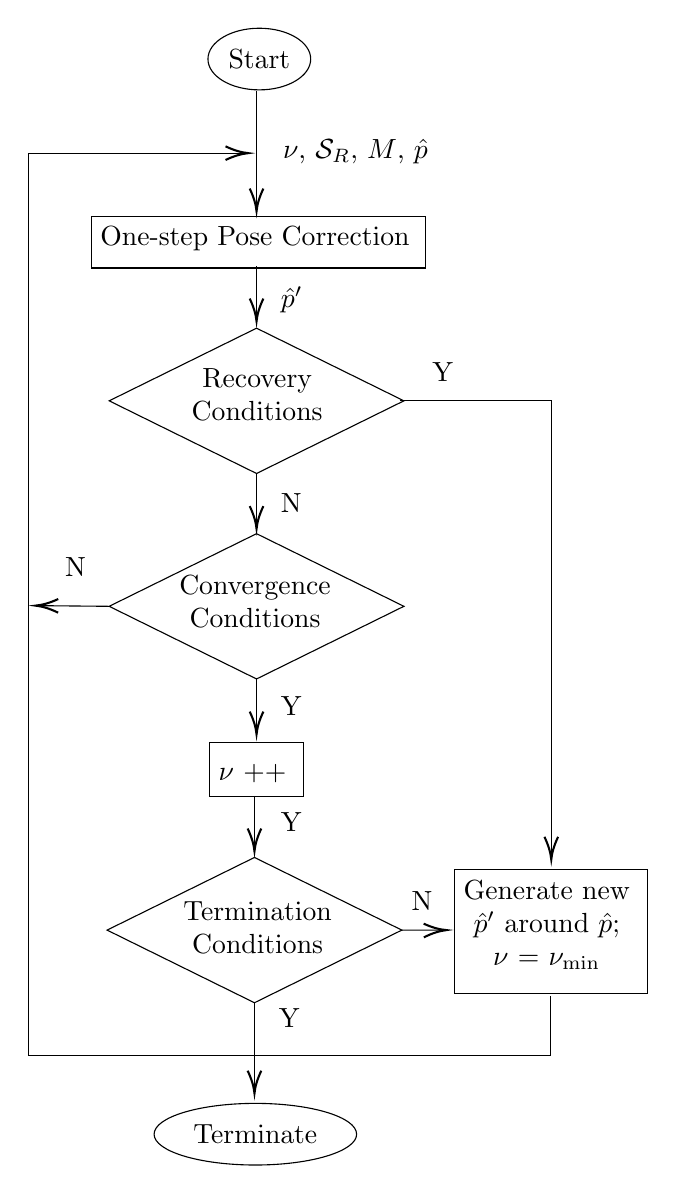
\begin{tikzpicture}[x=0.75pt,y=0.75pt,yscale=-1,xscale=1]
%uncomment if require: \path (0,1001); %set diagram left start at 0, and has height of 1001

%Flowchart: Decision [id:dp5485531374796404]
\draw   (240.5,167) -- (311.5,202) -- (240.5,237) -- (169.5,202) -- cycle ;
%Straight Lines [id:da5877536487984554]
\draw    (240.5,52.67) -- (240.5,108.67) ;
\draw [shift={(240.5,110.67)}, rotate = 270] [color={rgb, 255:red, 0; green, 0; blue, 0 }  ][line width=0.75]    (10.93,-3.29) .. controls (6.95,-1.4) and (3.31,-0.3) .. (0,0) .. controls (3.31,0.3) and (6.95,1.4) .. (10.93,3.29)   ;
%Straight Lines [id:da7274819726754627]
\draw    (240.5,237) -- (240.5,261.67) ;
\draw [shift={(240.5,263.67)}, rotate = 270] [color={rgb, 255:red, 0; green, 0; blue, 0 }  ][line width=0.75]    (10.93,-3.29) .. controls (6.95,-1.4) and (3.31,-0.3) .. (0,0) .. controls (3.31,0.3) and (6.95,1.4) .. (10.93,3.29)   ;
%Straight Lines [id:da7064477442798851]
\draw    (309.5,202) -- (382.5,202) -- (382.5,422) ;
\draw [shift={(382.5,423)}, rotate = 270.0] [color={rgb, 255:red, 0; green, 0; blue, 0 }  ][line width=0.75]    (10.93,-3.29) .. controls (6.95,-1.4) and (3.31,-0.3) .. (0,0) .. controls (3.31,0.3) and (6.95,1.4) .. (10.93,3.29)   ;
%Flowchart: Decision [id:dp1133428099178595]
\draw   (240.5,266) -- (311.5,301) -- (240.5,336) -- (169.5,301) -- cycle ;
%Flowchart: Decision [id:dp5073654995853492]
\draw   (239.5,422) -- (310.5,457) -- (239.5,492) -- (168.5,457) -- cycle ;
%Straight Lines [id:da1335991408375894]
\draw    (239.5,492) -- (239.5,533.67) ;
\draw [shift={(239.5,535.67)}, rotate = 270] [color={rgb, 255:red, 0; green, 0; blue, 0 }  ][line width=0.75]    (10.93,-3.29) .. controls (6.95,-1.4) and (3.31,-0.3) .. (0,0) .. controls (3.31,0.3) and (6.95,1.4) .. (10.93,3.29)   ;
%Straight Lines [id:da5471544644867792]
\draw    (234.5,82.67) -- (130.5,82.67) -- (130.5,517.33) ;
\draw [shift={(236.5,82.67)}, rotate = 180] [color={rgb, 255:red, 0; green, 0; blue, 0 }  ][line width=0.75]    (10.93,-3.29) .. controls (6.95,-1.4) and (3.31,-0.3) .. (0,0) .. controls (3.31,0.3) and (6.95,1.4) .. (10.93,3.29)   ;
%Straight Lines [id:da06493806045400974]
\draw    (310.5,457) -- (329,457.03) -- (332,457.03) ;
\draw [shift={(332,457)}, rotate = 539.01] [color={rgb, 255:red, 0; green, 0; blue, 0 }  ][line width=0.75]    (10.93,-3.29) .. controls (6.95,-1.4) and (3.31,-0.3) .. (0,0) .. controls (3.31,0.3) and (6.95,1.4) .. (10.93,3.29)   ;
%Straight Lines [id:da02699596164541651]
\draw    (240.5,137) -- (240.5,161.67) ;
\draw [shift={(240.5,163.67)}, rotate = 270] [color={rgb, 255:red, 0; green, 0; blue, 0 }  ][line width=0.75]    (10.93,-3.29) .. controls (6.95,-1.4) and (3.31,-0.3) .. (0,0) .. controls (3.31,0.3) and (6.95,1.4) .. (10.93,3.29)   ;
%Straight Lines [id:da5283272652442879]
\draw    (240.5,336) -- (240.5,360.67) ;
\draw [shift={(240.5,362.67)}, rotate = 270] [color={rgb, 255:red, 0; green, 0; blue, 0 }  ][line width=0.75]    (10.93,-3.29) .. controls (6.95,-1.4) and (3.31,-0.3) .. (0,0) .. controls (3.31,0.3) and (6.95,1.4) .. (10.93,3.29)   ;
%Straight Lines [id:da11468273552980146]
\draw    (239.5,392.33) -- (239.5,417) ;
\draw [shift={(239.5,419)}, rotate = 270] [color={rgb, 255:red, 0; green, 0; blue, 0 }  ][line width=0.75]    (10.93,-3.29) .. controls (6.95,-1.4) and (3.31,-0.3) .. (0,0) .. controls (3.31,0.3) and (6.95,1.4) .. (10.93,3.29)   ;
%Straight Lines [id:da44842589807001]
\draw    (169.5,301) -- (136,300.69) ;
\draw [shift={(134,300.67)}, rotate = 360.53999999999996] [color={rgb, 255:red, 0; green, 0; blue, 0 }  ][line width=0.75]    (10.93,-3.29) .. controls (6.95,-1.4) and (3.31,-0.3) .. (0,0) .. controls (3.31,0.3) and (6.95,1.4) .. (10.93,3.29)   ;
%Straight Lines [id:da5521661750319236]
\draw    (382,488.67) -- (382,517.33) -- (130.5,517.33) ;

% Text Node
\draw    (161,113) -- (322,113) -- (322,138) -- (161,138) -- cycle  ;
\draw (164,117) node [anchor=north west][inner sep=0.75pt]   [align=center] {One-step Pose Correction};
% Text Node
\draw    (241.84, 37.33) circle [x radius= 24.75, y radius= 14.85]   ;
\draw (241.84,37.33) node   [align=left] {Start};
% Text Node
\draw (208,185) node [anchor=north west][inner sep=0.75pt]  [align=center] {Recovery\\Conditions};
% Text Node
\draw (202,285) node [anchor=north west][inner sep=0.75pt]  [align=center] {Convergence\\Conditions};
% Text Node
\draw    (336,427.67) -- (429,427.67) -- (429,487.67) -- (336,487.67) -- cycle  ;
\draw (339,431.67) node [anchor=north west][inner sep=0.75pt]  [align=center] {Generate new \\ $\hat{\bm{p}}^\prime$ around $\hat{\bm{p}}$; \\ $\nu$ = $\nu_{\min}$};
% Text Node
\draw (324,182.33) node [anchor=north west][inner sep=0.75pt]   [align=left] {Y};
% Text Node
\draw (251,245.33) node [anchor=north west][inner sep=0.75pt]   [align=left] {N};
% Text Node
\draw    (218,366.67) -- (263,366.67) -- (263,392.67) -- (218,392.67) -- cycle  ;
\draw (221,375.67) node [anchor=north west][inner sep=0.75pt]   [align=center] {$\nu$ ++};
% Text Node
\draw (251,343.33) node [anchor=north west][inner sep=0.75pt]   [align=left] {Y};
% Text Node
\draw (252,74.57) node [anchor=north west][inner sep=0.75pt]   [align=left] {$\nu$, $\mathcal{S}_R$, $\bm{M}$, $\hat{\bm{p}}$};
% Text Node
\draw (204,442) node [anchor=north west][inner sep=0.75pt] [align=center] {Termination\\Conditions};
% Text Node
\draw    (239.93, 555.33) circle [x radius= 48.79, y radius= 14.85]   ;
\draw (239.93,555.33) node   [align=left] {Terminate};
% Text Node
\draw (147,276.33) node [anchor=north west][inner sep=0.75pt]   [align=left] {N};
% Text Node
\draw (251,399.33) node [anchor=north west][inner sep=0.75pt]   [align=left] {Y};
% Text Node
\draw (314,437.33) node [anchor=north west][inner sep=0.75pt]   [align=left] {N};
% Text Node
\draw (251,145.57) node [anchor=north west][inner sep=0.75pt]   [align=left] {$\hat{\bm{p}}^\prime$};
% Text Node
\draw (250,493.33) node [anchor=north west][inner sep=0.75pt]   [align=left] {Y};


\end{tikzpicture}


      \end{figure}
    \end{minipage}
  \end{minipage}
  }


\note{\footnotesize
Με την εισαγωγή της μετρικής CAER μπορούμε τώρα να συνθέσουμε το τελικό σύστημα
που επιλύει το πρόβλημα sm2 χωρίς αντιστοιχίσεις. Δεδομένων των παραδοχών του
προβλήματος, το σύστημα fsm2 ελαττώνει επαναληπτικά το σφάλμα στάσης με τον
εξης τροπο. Αρχικά πραγματοποιείται εκτίμηση του προσανατολισμού, η οποία
παράγει 2 εις την ν εκτιμήσεις στάσης, όλες με την ίδια θέση αλλα
διαφορετικό προσανατολισμό.  Στη συνέχεια κάθε εκτίμηση
οδευεται στο σύστημα εκτίμησης θέσης για μία επανάληψη, και σε αυτό το στάδιο
παράγονται 2 εις την ν εκτιμήσεις στάσης, όλες με διαφορετικό προσανατολισμό
και θέση. Με αυτόν τον τρόπο εκτιμήσεις που έχουν μεγαλύτερο σφάλμα
προσανατολισμού αποκτούν ακόμα μεγαλύτερο σφάλμα θέσης, και έτσι γίνεται
ευκολότερη η διάκριση της στάσης με το μικρότερο σφάλμα από τη μετρική CAER.
Στη συνέχεια υπολογίζεται η τιμή CAER για όλους τους συνδυασμούς της
πραγματικής σάρωσης με την εικονική σάρωση που προκύπτει από τις εκτιμήσεις,
και η έξοδος του συστήματος εκτίμησης προσανατολισμού θεωρείται εκείνη που
παράγει την ελάχιστη τιμή CAER. Στη συνέχεια αυτή η εκτίμηση στάσης οδεύεται
στο σύστημα εκτίμησης θέσης, και η διαδικασία επαναλαμβάνεται με βάση αυτή την
εκτίμηση εως ότου ικανοποιηθεί μια σειρά συνθηκών σύγκλισης και τερματισμού.}


\end{frame}
